\documentclass[a4paper]{article}
\usepackage[utf8]{inputenc}
\usepackage[spanish, es-tabla, es-noshorthands]{babel}
\usepackage[table,xcdraw]{xcolor}
\usepackage[a4paper, footnotesep = 1cm, width=20cm, top=2.5cm, height=25cm, textwidth=18cm, textheight=25cm]{geometry}
%\geometry{showframe}

\usepackage{tikz}
\usepackage{amsmath}
\usepackage{amsfonts}
\usepackage{amssymb}
\usepackage{float}
\usepackage{graphicx}
\usepackage{caption}
\usepackage{subcaption}
\usepackage{multicol}
\usepackage{multirow}
\setlength{\doublerulesep}{\arrayrulewidth}
\usepackage{booktabs}
\usepackage{mathrsfs,amsmath}
\usepackage{hyperref}
\hypersetup{
    colorlinks=true,
    linkcolor=blue,
    filecolor=magenta,      
    urlcolor=blue,
    citecolor=blue,    
}

\newcommand{\quotes}[1]{``#1''}
\usepackage{array}
\newcolumntype{C}[1]{>{\centering\let\newline\\\arraybackslash\hspace{0pt}}m{#1}}
\usepackage[american]{circuitikz}
\usetikzlibrary{calc}
\usepackage{fancyhdr}
\usepackage{units} 

\graphicspath{./Imagenes}

\pagestyle{fancy}
\fancyhf{}
\lhead{22.05 ASSD}
\rhead{Mechoulam, Lambertucci, Rodriguez, Londero}
\rfoot{Página \thepage}

\begin{document}

\subsection{Realización de espectrograma}

Los espectrogramas son gráficos que muestras la evolución del espectro de una señal conforme pasa el tiempo. Estos son de gran utilidad en el campo de las telecomunicaciones, speech processing, geología terrestre, entre otros.

\subsubsection{Solapamiento y la necesidad de ver más detalle}
En alguna aplicaciones, como es en el caso de las telecomunicaciones, las señales pueden sufrir cambios en la frecuencia de portadora en intervalos de tiempo muy cortos como es el caso de \textbf{frequency hopping} en el caso del desarrollo de señales de espectro expandido en el cual se efectúan saltos en frecuencia de portadora controlados. Principalmente se utiliza para evitar interferencia con otros dispositivos.

Cuando se estudian este tipo de señales es necesario conseguir una resolución temporal muy fina con el fin de ver eventos de duración extremadamente corta, en particular eventos que duran menos que el tamaño de un bloque. Un espectrograma tradicional, sin solapamiento, toma la señal de a bloques y procede a computar el espectro correspondiente. Sin embargo los bloques subsiguientes ignoran por completo la historia pasada de la señal. Para poder mejorar la resolución temporal y recuperar eventos de corta duración se aplica la técnica de solapamiento. Se debe tener cierto cuidado con la terminología dado que este método no realiza un acercamiento, "zoom", en el eje temporal sino que más bien aumenta su la cantidad de puntos intermedios disponibles. 
  
\begin{figure}[H]
	\centering
	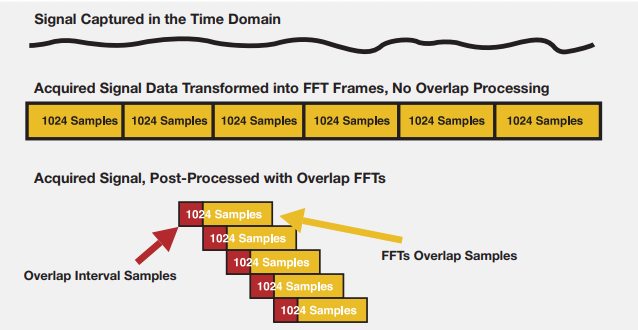
\includegraphics[width=0.7\linewidth]{ImagenesEjercicio7/OverlapDiagram}
	\caption{Esquema de solapamiento}
	\label{fig:overlapdiagram}
\end{figure}

Este método ralentiza significativamente el tiempo de computo del espectrograma al aumentar la cantidad de FFTs a realizar.

En las figura debajo podemos observar como, a medida que aumenta el solapamiento, se hacen visibles los hops en frecuencia que hace la señal.
\begin{figure}[H]
	\centering
	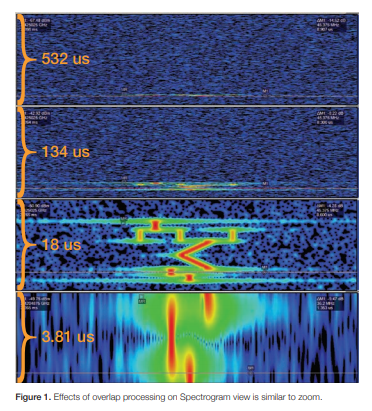
\includegraphics[width=0.7\linewidth]{ImagenesEjercicio7/Zoooom}
	\caption{Saltos en frecuencia con solapamiento}
	\label{fig:zoooom}
\end{figure}



\begin{figure}[H]
	\centering
	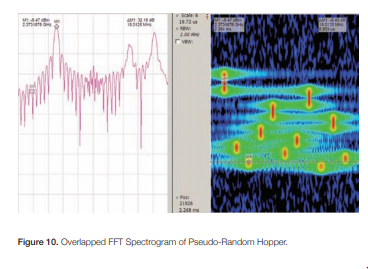
\includegraphics[width=0.7\linewidth]{ImagenesEjercicio7/Zoooom2}
	\caption{Visualización de Frequency Hopping Spread Spectrum}
	\label{fig:zoooom2}
\end{figure}


\subsubsection{Espectograma de la escala G3(sol mayor)}
Para la realización de este espectrograma se compuso un archivo \textit{MIDI} utilizando el programa de procesamiento de audio \textit{Audacity} y se utilizo el programa desarrollado para componer la pista de audio con su correspondiente espectograma.

\begin{figure}[H]
	\centering
	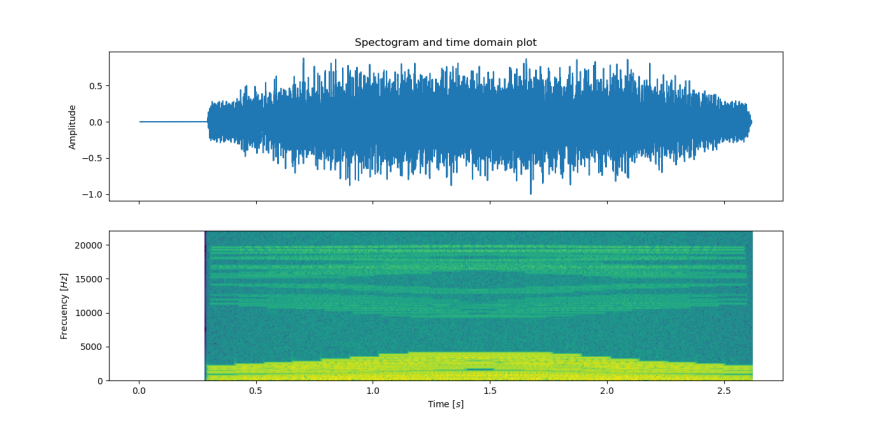
\includegraphics[width=0.7\linewidth]{ImagenesEjercicio7/EspectogramaOrganoEscala}
	\caption{Espectrograma Organo}
	\label{fig:espectogramaorganoescala}
\end{figure}
Los parámetros utilizados para la ventana del organo fueron
a = 0.05, h = 0.01, r = 0.1.
\subsubsection{Bibliografia}
Para la realización de esta sección se hizo uso de documentación tecnica publicada por Tektronix: \textit{Understanding FFT Overlap Processing
A Tektronix Real-Time Spectrum Analyzer Primer} y 
\end{document}